En este capítulo estudiamos el rol de la interacción de Coulomb en la dinámica de los nucleones en las condiciones de la corteza de las estrellas de neutrones.
Estudiamos la materia simétrica en isospín a densidades de sub-saturación y temperaturas bajas.
La interacción electrostática entre protones es incluida como un potencial de Coulomb apantallado, en el espíritu de la aproximación de Thomas-Fermi, pero variando artificialmente la longitud de apantallamiento para estudiar su efecto en la formación de las estructuras nucleares no homogéneas conocidas como ``pasta nuclear''.
A medida que aumenta la longitud de apantallamiento, podemos ver una transición de un régimen de una pasta por celda (debido exclusivamente a efectos de tamaño finito) a un régimen en el que aparecen múltiples pastas por celda.
Esta diferencia cualitativa en la estructura de la materia de estrellas de neutrones a bajas temperaturas muestra que se debe tomar especial cuidado cuando la longitud de apantallamiento es estimada para simulaciones numéricas.

Como observamos en trabajos previos~\cite{schneider_nuclear_2013,gimenez_molinelli_simulations_2014}, en ausencia de la interacción de Coulomb (equivalente a $\lambda=0$), estructuras tipo pastas pueden ser observadas, aunque sólo una por celda.
Estas \emph{pseudo-pastas} también tienen formas de esferas, tubos, placas, anti-tubos y anti-esferas, exactamente como la pasta con la interacción de Coulomb.
La mayor diferencia es que, sin la interacción de Coulomb, encontramos siempre una estructura por celda, lo que nos hace pensar que la estructura está relacionada con la condición periódica de contorno impuesta en la caja,
La \emph{pseudo-pasta} existe debido a efectos de tamaño finito y, si la caja no existiera, la solución sería una gota infinita.
Notamos, sin embargo, que cuando existe la interacción de Coulomb, la competencia entre interacciones opuestas genera una longitud característica, ya no relacionada con el tamaño de la caja.
A densidades de sub-saturación esta competencia es responsable por las fases de pasta, y en el límite de densidades muy bajas le da forma a los núcleos a los que estamos acostumbrados.

Incrementar el valor de $\lambda$ comenzando desde $0\,\text{fm}$, apuntamos a explorar la transición de las pastas artificiales en las que se produce una estructura por celda hacia las pastas más realistas que tienen múltiples estructuras en cada celda de simulación.
Más aún, esto nos permite estudiar las implicancias físicas del valor arbitrario y utilizado tradicionalmente de $\lambda=10\,\text{fm}$.

\section{Introducción}

En las estrellas de neutrones, además de los protones y neutrones, existe un gas de electrones que permea todo el espacio.
Este gas de electrones apantalla la interacción electrostática de rango largo entre los protones.
Este efecto de apantallamiento es usualmente modelado con la aproximación de Thomas-Fermi, de acuerdo a la cual la interacción entre protones es un potencial del tipo Yukawa con una longitud de apantallamiento $\lambda$, conocida como longitud de Debye:

\begin{equation*}
 V_{TF}(r) = \text{q}^2\frac{e^{-r/\lambda}}{r}
\end{equation*}

De acuerdo a cálculos de Teoría Cuántica de Campos~\cite[pp. 175-180]{fetter_quantum_2003}, la longitud de apantallamiento a las densidades de interés es $\lambda\approx100\,\text{fm}$. 
Para simulaciones numéricas una interacción de rango tan largo implica un problema ya que, para realizar simulaciones correctas, el dominio de la simulación debería ser mayor que la longitud de los potenciales de interacción.
El valor correcto de $\lambda$ requeriría trabajar con $\approx 10^6$ partículas, y sería muy complicado de realizar computacionalmente.
Al enfrentar este inconveniente, distintos autores~\cite{maruyama_molecular_2012, horowitz_neutrino-pasta_2004} decidieron trabajar con un valor mucho menor $\lambda=10\,\text{fm}$, con la esperanza de retener los principales aspectos cualitativos y fenomenológicos del sistema (interacciones competitivas de distinto rango) al trabajar con sistemas más pequeños.
Incluso si fueran capaces de producir estructura del tipo pasta, la elección particular del valor para la longitud de apantallamiento es arbitraria y basada casi únicamente en detalles computacionales.
Notablemente, este valor de longitud de apantallamiento fue utilizado
consecutivamente por los autores desde ese momento~\cite{maruyama_quantum_1998, horowitz_neutrino-pasta_2004, dorso_topological_2012}.
En este capítulo nos centraremos en el estudio de las consecuencias física de esta elección arbitraria.

El rol de la longitud de apantallamiento ha sido apenas explorado en otros modelos.
Por ejemplo, en un estudio del 2003~\cite{watanabe_electron_2003}, el efecto de apantallamiento de un gas de electrones en estructuras nucleares fue investigado utilizando un modelo estático de gota líquida.
En este estudio se encontró que el principal efecto del gas apantallante fue extender el rango de densidades en las que las burbujas y los fragmentos aparecían, y reducir el rango de estabilidad de fases homogéneas.
A pesar de que la relevancia del apantallamiento resultó menor, el estudio, al ser estático, no incluía ningún efecto dinámico.

Otro estudio, del 2005~\cite{maruyama_nuclear_2005}, utilizó una funcional densidad para investigar el apantallamiento de la carga en estructuras nucleares a densidades menores a la nuclear, pero a temperatura cero; en particular se compararon casos con y sin apantallamiento.
Los resultados principales del estudio fueron perfiles de densidad de nucleones utilizados para cuantificar el ordenamiento de las densidades de carga de protones y electrones.
Nuevamente, hallaron que las regiones de densidad en las que existe la pasta se amplían cuando se considera el apantallamiento de Coulomb, especialmente debido al reordenamiento de los protones; los autores remarcan la importancia de extender este estudio a temperaturas finitas y con modelos dinámicos.

Más recientemente, algunos trabajos~\cite{schneider_nuclear_2013,gimenez_molinelli_simulations_2014} comenzaron a estudiar el efecto que tiene la interacción de Coulomb en la formación de pasta utilizando modelos dinámicos.
Los hallazgos principales fueron que la pasta artificial, de una estructura por celda (\emph{pseudo-pasta}), podía existir incluso en ausencia de interacción de Coulomb, y que existía debido a las condiciones periódicas de contorno y el tamaño finito~\cite{binder_beyond_2012}.

\section{Longitud de apantallamiento ``crítica''}\label{lambda_c}

Una forma de analizar la naturaleza de la pasta obtenida es a través de la presión de las distintas configuraciones.

Podemos medir la presión a través de la fórmula del virial
\begin{equation*}
P=\frac{N\,k_B\,T}{V} + \frac{1}{3}
\frac{\Sigma_{i}^{N}\mathbf{r}_i\cdot\mathbf{F}_i}{V}
\end{equation*}
donde $N$ es el número de partículas en el sistema y $\mathbf{F}$ la fuera ejercida sobre cada nucleón.
Los términos en la fórmula del virial se aplican sólo a las interacciones específicas del modelo, sin contemplar la presión del gas de electrones.
Esta presión no debe ser confundida con la presión esperada en la corteza de las estrellas de neutrones (ya que los electrones deberían ser considerados explícitamente para calcularla adecuadamente), sino simplemente una prueba de la estabilidad mecánica de las configuraciones obtenidas con este modelo.
En la figura~\ref{fig:pre} vemos que para todo $\lambda<10\,\text{fm}$ la presión es negativa.

La presión negativa es una señal de que las estructuras no-homogéneas encontradas son artificiales, y que las estructuras sólo pueden existir bajo condiciones periódicas de contorno (ver~\cite{binder_beyond_2012,gimenez_molinelli_simulations_2014}).
Podemos pensar al sistema como la celda primitiva de la simulación bajo la tensión causada por sus réplicas periódicas.
Esto significa que, para longitudes de apantallamiento tan bajas, la interacción efectiva es atractiva y las condiciones periódicas de contorno todavía juegan un rol importante en la forma del estado de mínima energía.

Para $\lambda>10\,\text{fm}$ la presión se vuelve positiva, lo que quiere decir que las estructuras que se forman en estas configuraciones no se deben sólo a las condiciones periódicas de contorno, sino que la interacción de Coulomb está comenzando a jugar un rol.
Las configuraciones para estos valores de $\lambda$ muestran efectivamente fluctuaciones de densidad de longitud menor que el tamaño de la caja, que sólo pueden ser atribuidas a la competencia entre el término de Coulomb y el término nuclear.
Sin embargo, la forma de las estructuras, caracterizadas a través de las funcionales de Minkowski, cambia drásticamente con $\lambda$.

\begin{figure}[h!]  \centering
\centering
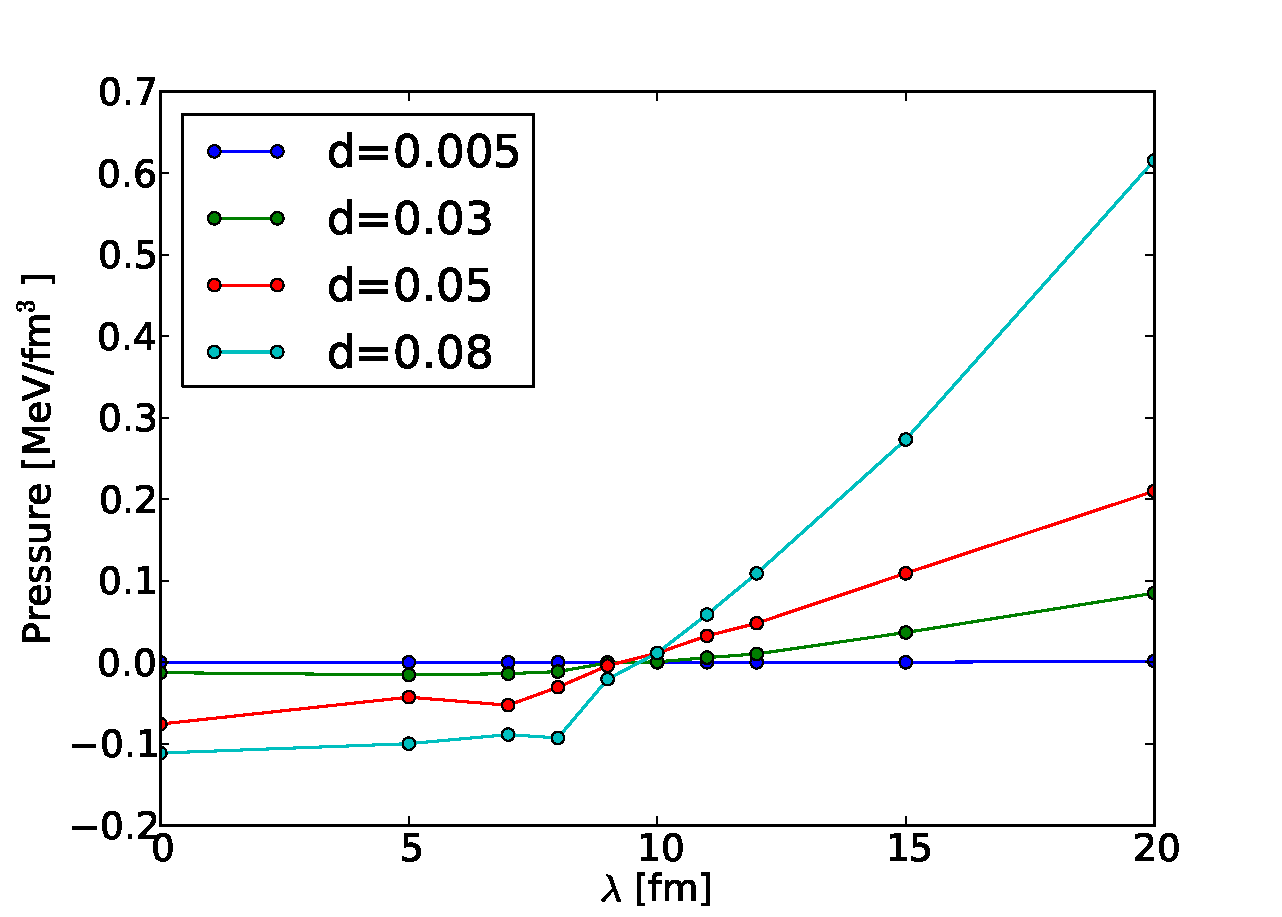
\includegraphics[width=0.7\columnwidth]{coulomb/pre.pdf}
\caption{Presión como función del apantallamiento $\lambda$ para distintas densidades.
  Podemos ver que para $\lambda<10\,\text{fm}$ la presión es negativa, sugiriendo que las condiciones periódicas de contorno están afectando la topología de la solución.}
\label{fig:pre}
\end{figure}

Para clasificar las estructuras de bajas temperaturas ($T=0.001\,\text{MeV}$) para cada valor de $\lambda$, estudiamos su topología con las herramientas de análisis para la distribución espacial de partículas: las funcionales de Minkowski.
En las figuras~\ref{fig:minkowski} podemos ver la superficie, ancho medio y número de Euler para los estados hallados y su dependencia con $\lambda$ para distintas densidades.

\begin{figure}[h!]  %figure 5 \centering
\centering
\begin{subfigure}[h!]{0.45\columnwidth}
  \centering
  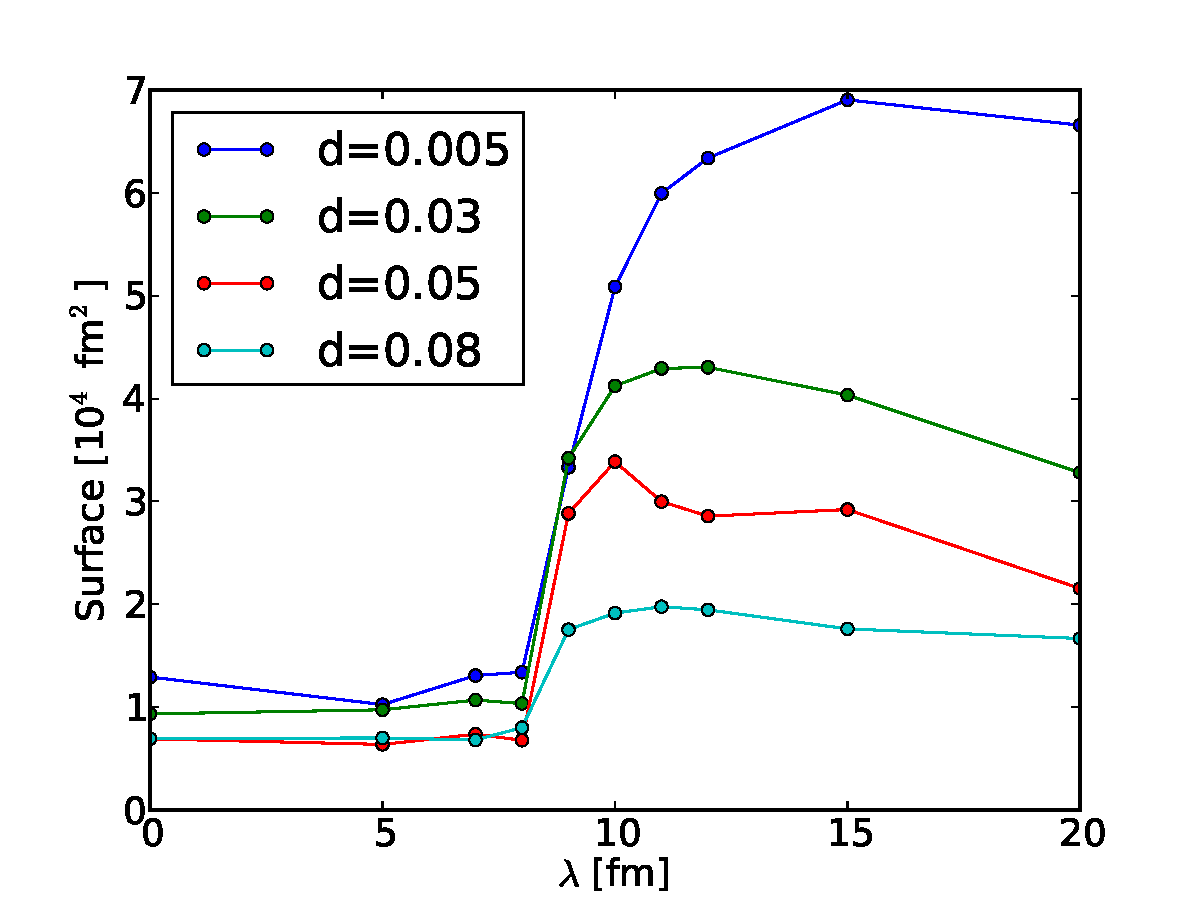
\includegraphics[width=\columnwidth]{coulomb/sup.pdf}
  \caption{Superficie}
\end{subfigure}
\begin{subfigure}[h!]{0.45\columnwidth}
  \centering
  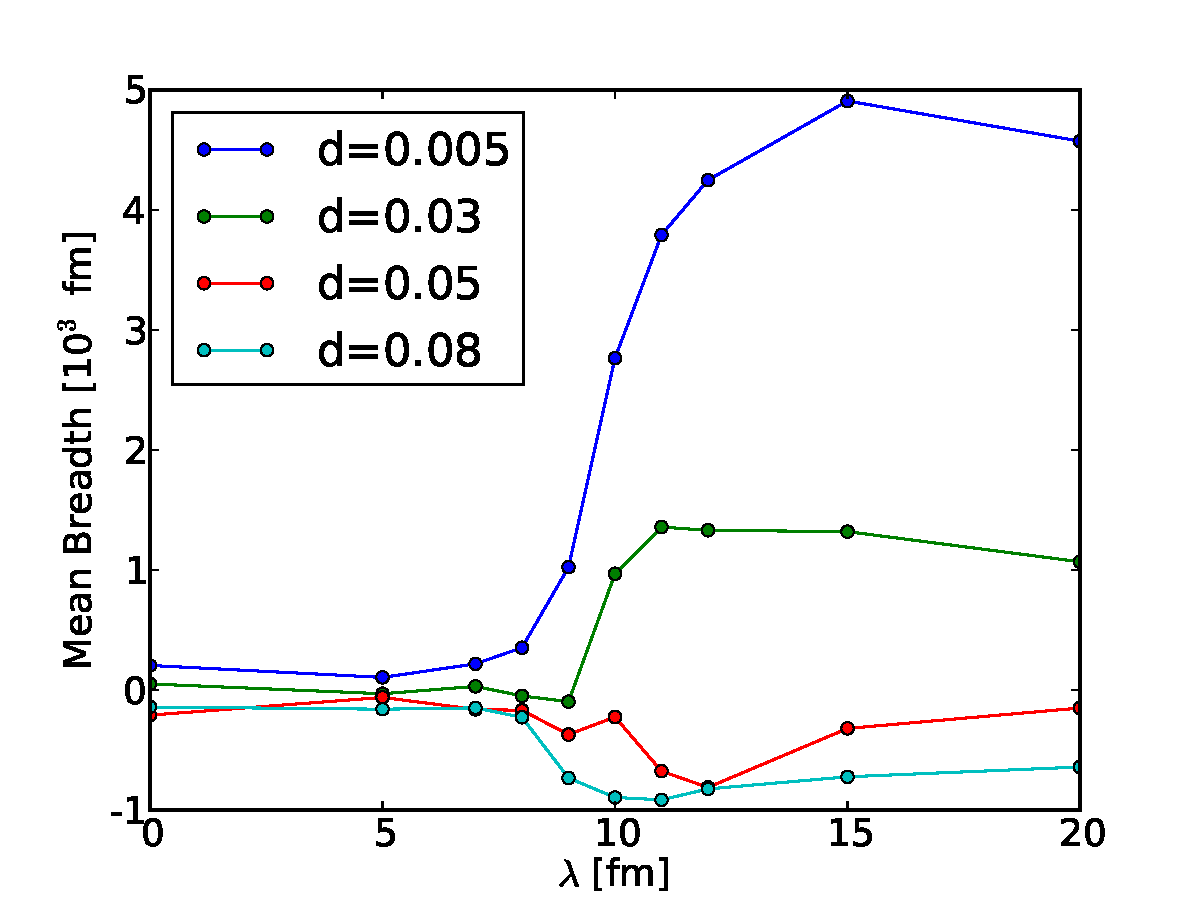
\includegraphics[width=\columnwidth]{coulomb/cur.pdf}
  \caption{Ancho medio}
\end{subfigure}
\begin{subfigure}[h!]{0.45\columnwidth}
  \centering
  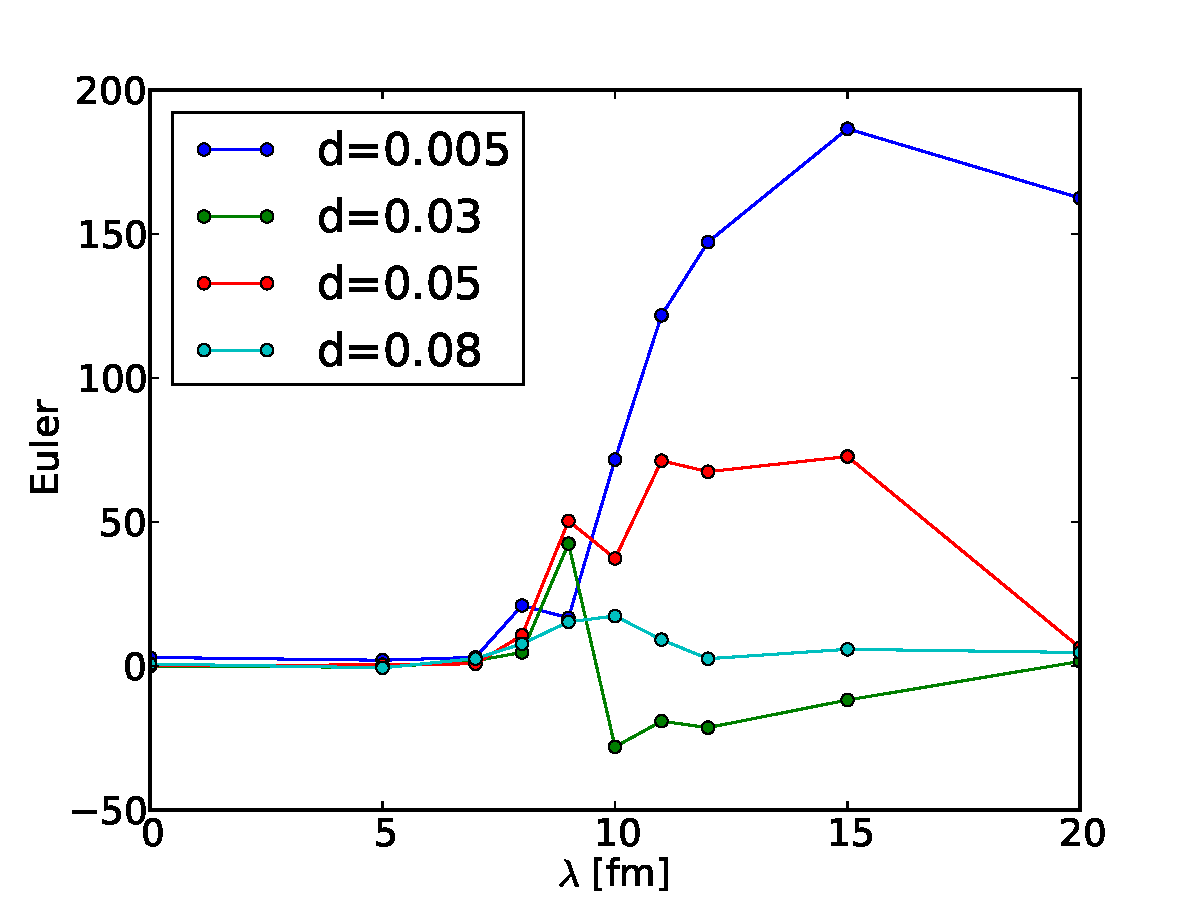
\includegraphics[width=\columnwidth]{coulomb/eul.pdf}
  \caption{Número de Euler}
\end{subfigure}
\caption{Dependencia de las funcionales de Minkowski con $\lambda$.
  Podemos observar un régimen de transición entre $\lambda=7\,\text{fm}$ y $\lambda=15\,\text{fm}$, donde las funcionales de Minkowski cambian.}
\label{fig:minkowski}
\end{figure}

\begin{table}[ht] \centering
\caption{Clasificación Ancho - Euler}
\begin{tabular}{c|| c | c | c} \hline & Ancho $<0$ & Ancho
$\sim 0$ & Ancho $>0$ \\
               
\hline\hline Euler $>0$ & Anti-Gnocchi (Burbujas) & & Gnocchi \\

Euler $\sim0$ & Anti-Spaghetti (Túneles) & Lasagna & Spaghetti \\

Euler $<0$ & Anti-Jungle Gym & & Jungle Gym \\ [1ex] \hline
\end{tabular}
\label{tab:mink}
\end{table}

Como se muestra en la tabla~\ref{tab:mink}, esperamos que \emph{lasagna} y \emph{spaghetti} tengan un número de Euler $\chi=0$.
Para el caso de los \emph{gnocchi}, sin embargo, cada uno de ellos contribuye con $\chi_{gn}=2$.
Esto significa que el número de Euler para todo el sistema de $N_{gn}$ \emph{gnocchi} será $\chi=2\cdot\,N_{gn}$.
A medida que las configuraciones se parten en múltiples estructuras por celda al aumentar $\lambda$, esperamos que también aumente la superficie.
En cuanto al ancho medio, el comportamiento descripto en la tabla~\ref{tab:mink} (positivo para \emph{spaghetti} y \emph{gnocchi}, cero para \emph{lasagna} y negativo para túnel sólo se observa para $\lambda=20\,\text{fm}$.
Entre $\lambda=7\,\text{fm}$ y $\lambda=10\,\text{fm}$ las tres funcionales de Minkowski cambian drásticamente antes de alcanzar valores bien definidos.
Esto indica que hay un régimen de transición en el que las estructuras no se pueden describir como cualquiera de las pastas tradicionales.
Para este modelo de interacción nuclear y Coulomb, parece que el valor usual de $\lambda=10\,\text{fm}$ es demasiado bajo.


\section{Régimen de una pasta por celda} \label{pasta-bup}

\begin{figure}
\centering
\begin{subfigure}[h!]{0.3\columnwidth}
  \centering
  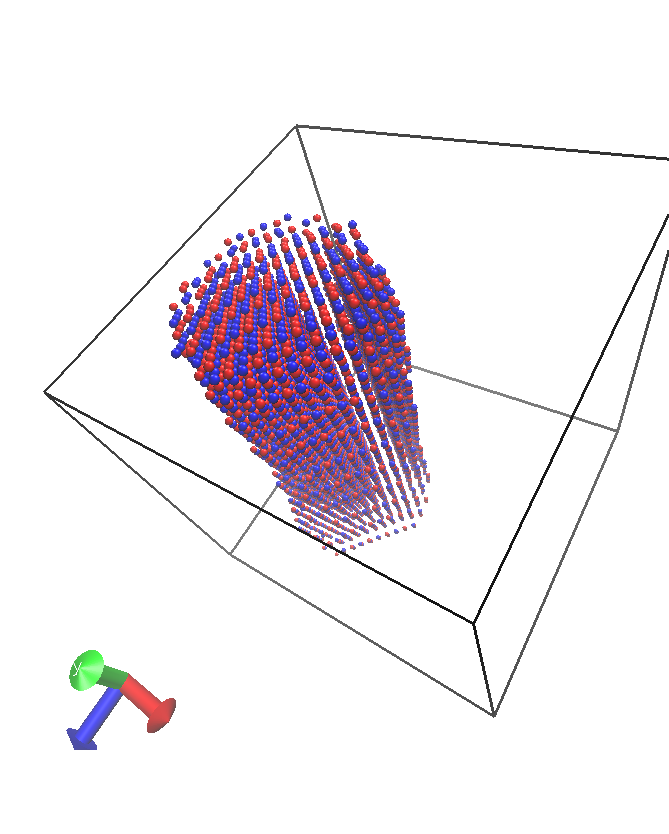
\includegraphics[width=\columnwidth]{coulomb/cou0-d0-03.png}
  \caption{$\rho=0.03\,\text{fm}^{-3}$, $\lambda=0\,\text{fm}$}
\end{subfigure}
\begin{subfigure}[h!]{0.3\columnwidth}
  \centering
  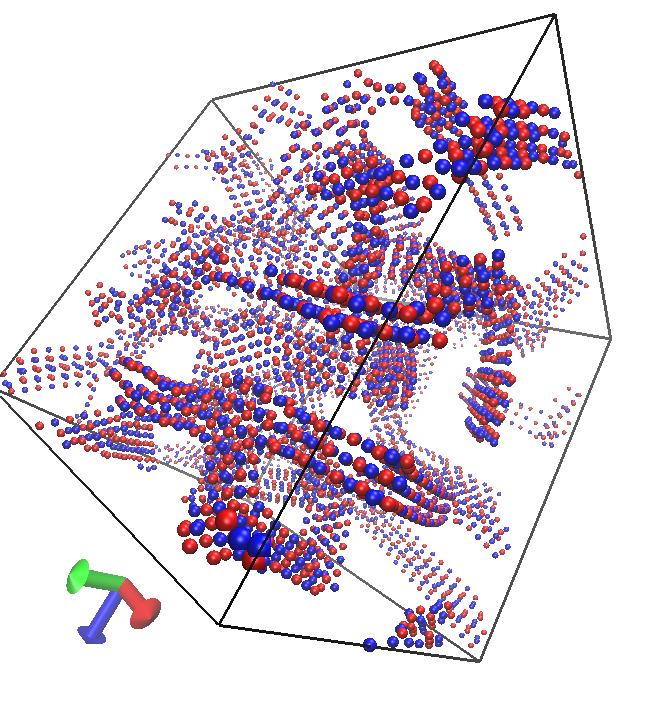
\includegraphics[width=\columnwidth]{coulomb/cou10-d0-03.png}
  \caption{$\rho=0.03\,\text{fm}^{-3}$, $\lambda=10\,\text{fm}$}
\end{subfigure}
\begin{subfigure}[h!]{0.3\columnwidth}
  \centering
  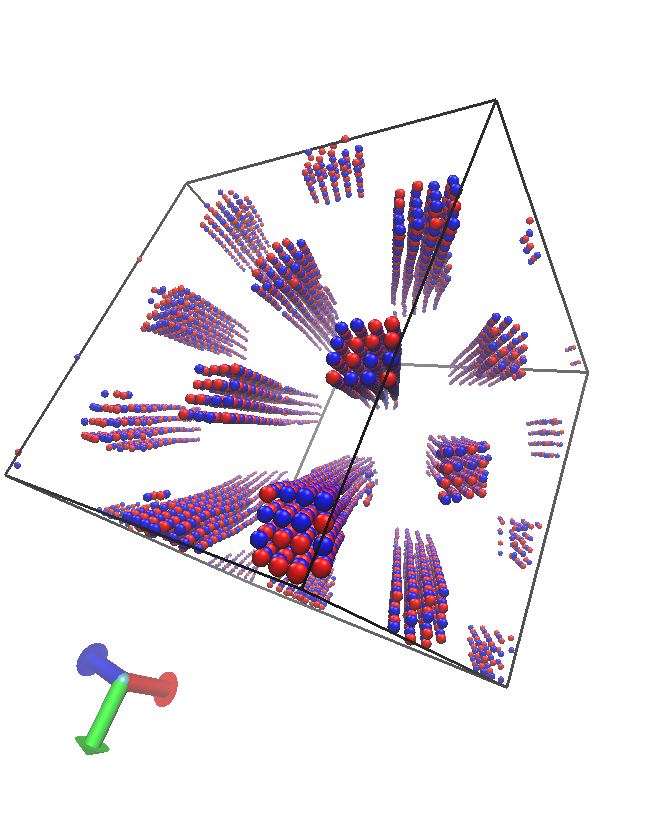
\includegraphics[width=\columnwidth]{coulomb/cou20-d0-03.png}
  \caption{$\rho=0.03\,\text{fm}^{-3}$, $\lambda=20\,\text{fm}$}
\end{subfigure}

\begin{subfigure}[h!]{0.3\columnwidth}
  \centering
  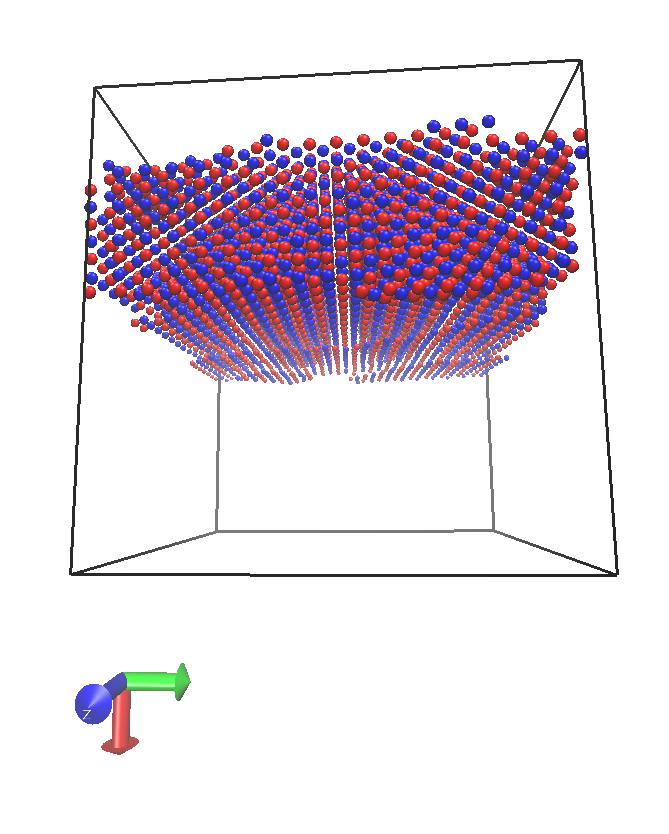
\includegraphics[width=\columnwidth]{coulomb/cou0-d0-05.png}
  \caption{$\rho=0.05\,\text{fm}^{-3}$, $\lambda=0\,\text{fm}$}
\end{subfigure}
\begin{subfigure}[h!]{0.3\columnwidth}
  \centering
  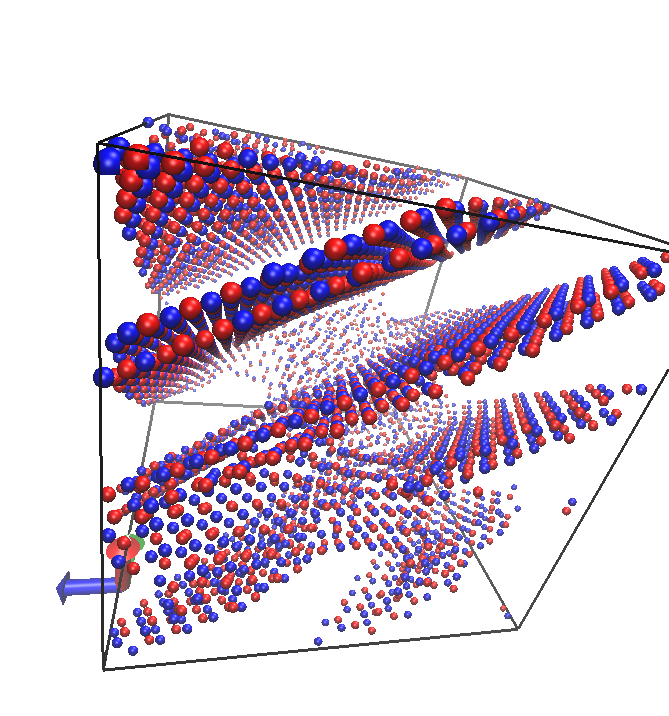
\includegraphics[width=\columnwidth]{coulomb/cou10-d0-05.png}
  \caption{$\rho=0.05\,\text{fm}^{-3}$, $\lambda=10\,\text{fm}$}
\end{subfigure}
\begin{subfigure}[h!]{0.3\columnwidth}
  \centering
  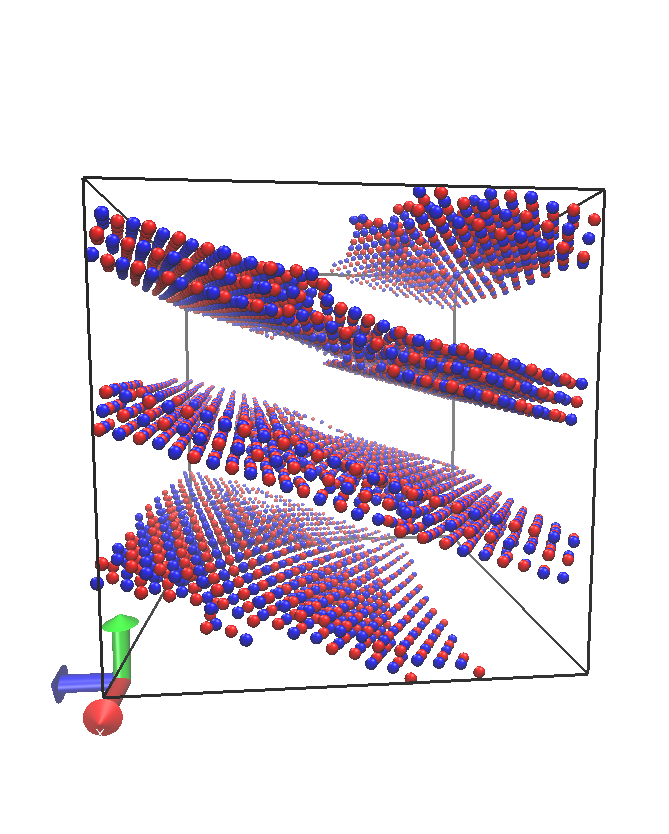
\includegraphics[width=\columnwidth]{coulomb/cou20-d0-05.png}
  \caption{$\rho=0.05\,\text{fm}^{-3}$, $\lambda=20\,\text{fm}$}
\end{subfigure}

\begin{subfigure}[h!]{0.3\columnwidth}
  \centering
  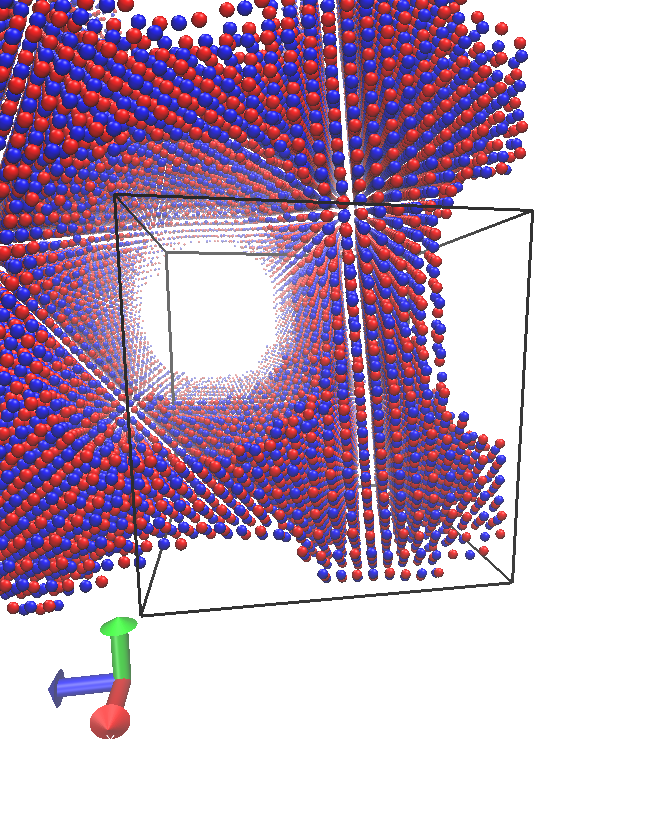
\includegraphics[width=\columnwidth]{coulomb/cou0-d0-08.png}
  \caption{$\rho=0.08\,\text{fm}^{-3}$, $\lambda=0\,\text{fm}$}
\end{subfigure}
\begin{subfigure}[h!]{0.3\columnwidth}
  \centering
  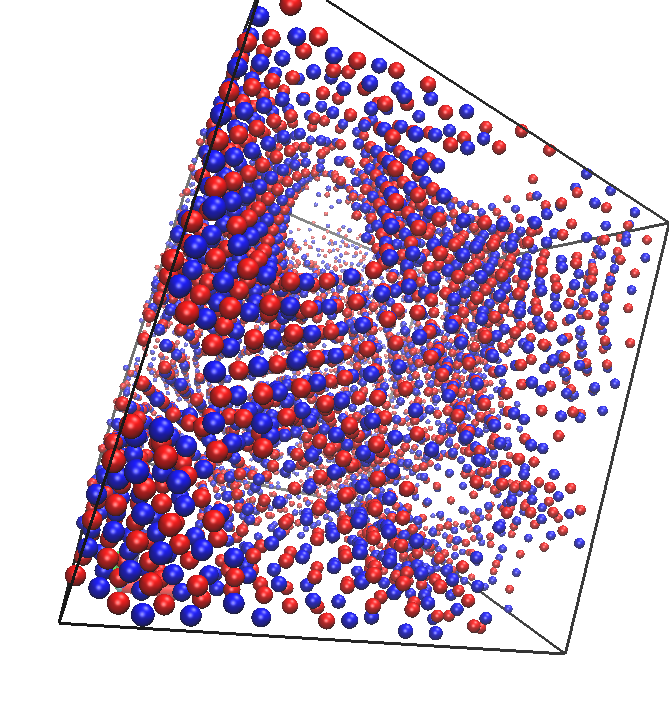
\includegraphics[width=\columnwidth]{coulomb/cou10-d0-08.png}
  \caption{$\rho=0.08\,\text{fm}^{-3}$, $\lambda=10\,\text{fm}$}
\end{subfigure}
\begin{subfigure}[h!]{0.3\columnwidth}
  \centering
  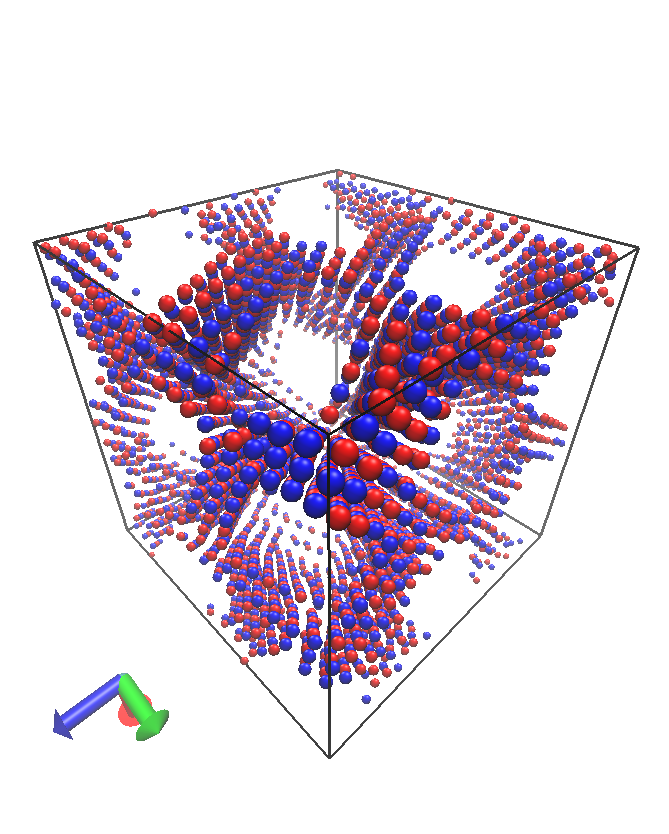
\includegraphics[width=\columnwidth]{coulomb/cou20-d0-08.png}
  \caption{$\rho=0.08\,\text{fm}^{-3}$, $\lambda=20\,\text{fm}$}
\end{subfigure}
\caption{Diferencia entre pasta con y sin interacción de Coulomb.
  Podemos ver que la interacción de Coulomb separa la pasta, convirtiendo una estructura por celda en múltiples estructuras por celda.}
\label{fig:w-wo-coulomb}
\end{figure}

Para comprender mejor cómo el estado de equilibrio a bajas temperaturas varía a través del régimen de transición desde la inexistencia de Coulomb hacia un apantallamiento de $\lambda=20\,\text{fm}$, mostramos en la figura~\ref{fig:w-wo-coulomb} representaciones visuales de los resultados obtenidos para un conjunto de densidades elegidos, con $\lambda=0$, $\lambda=10\,\text{fm}$ y $\lambda=20\,\text{fm}$.
Vemos que obtenemos estructuras exóticas para $\lambda=10\,\text{fm}$ en los tres casos, que son variaciones de la estructura típica de la pasta que pueden deberse al complicado paisaje de energías para estos valores de $\lambda$.

\begin{figure}[h!]  %figure 5 \centering
\centering
\begin{subfigure}[h!]{0.48\columnwidth}
  \centering
  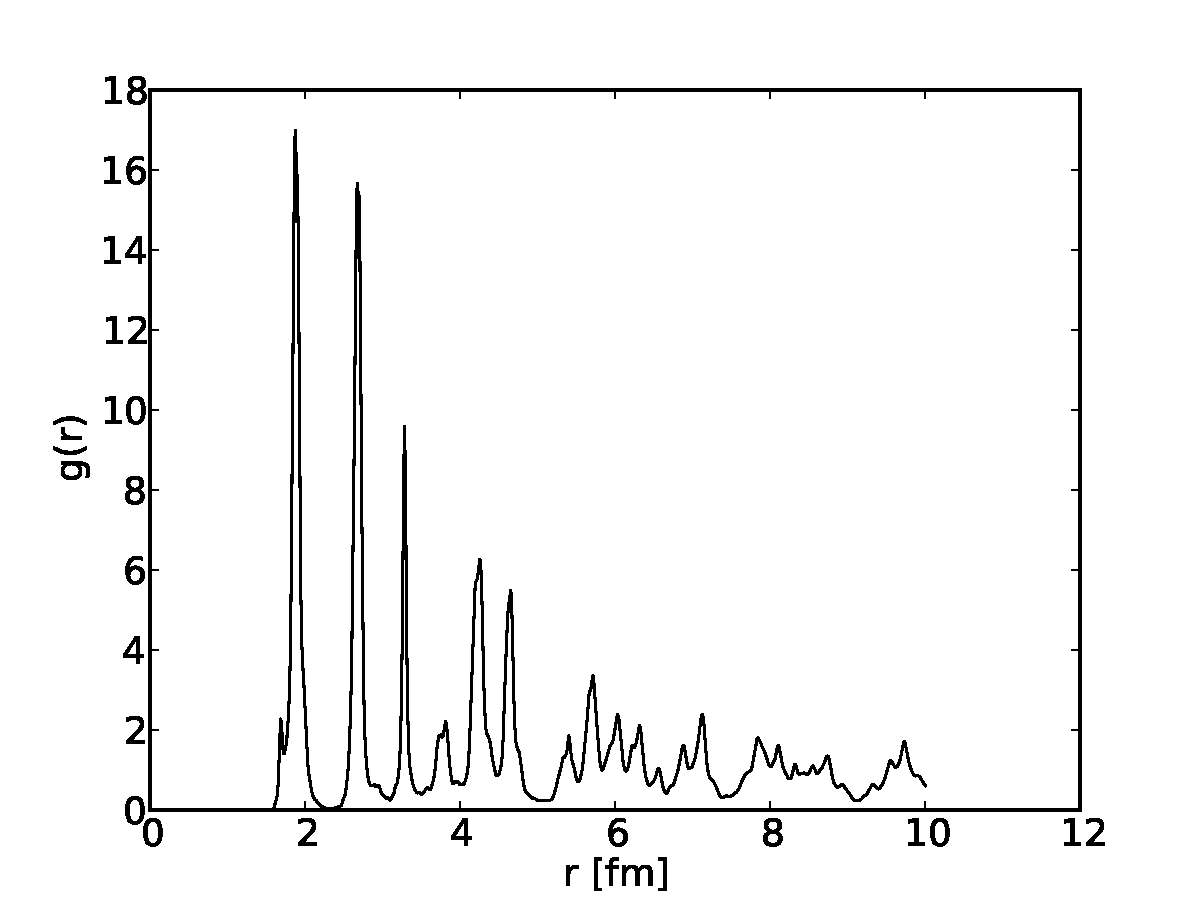
\includegraphics[width=\columnwidth]{coulomb/gofr-mult.pdf}
  \caption{Múltiples lasagnas}
\end{subfigure}
\begin{subfigure}[h!]{0.48\columnwidth}
  \centering
  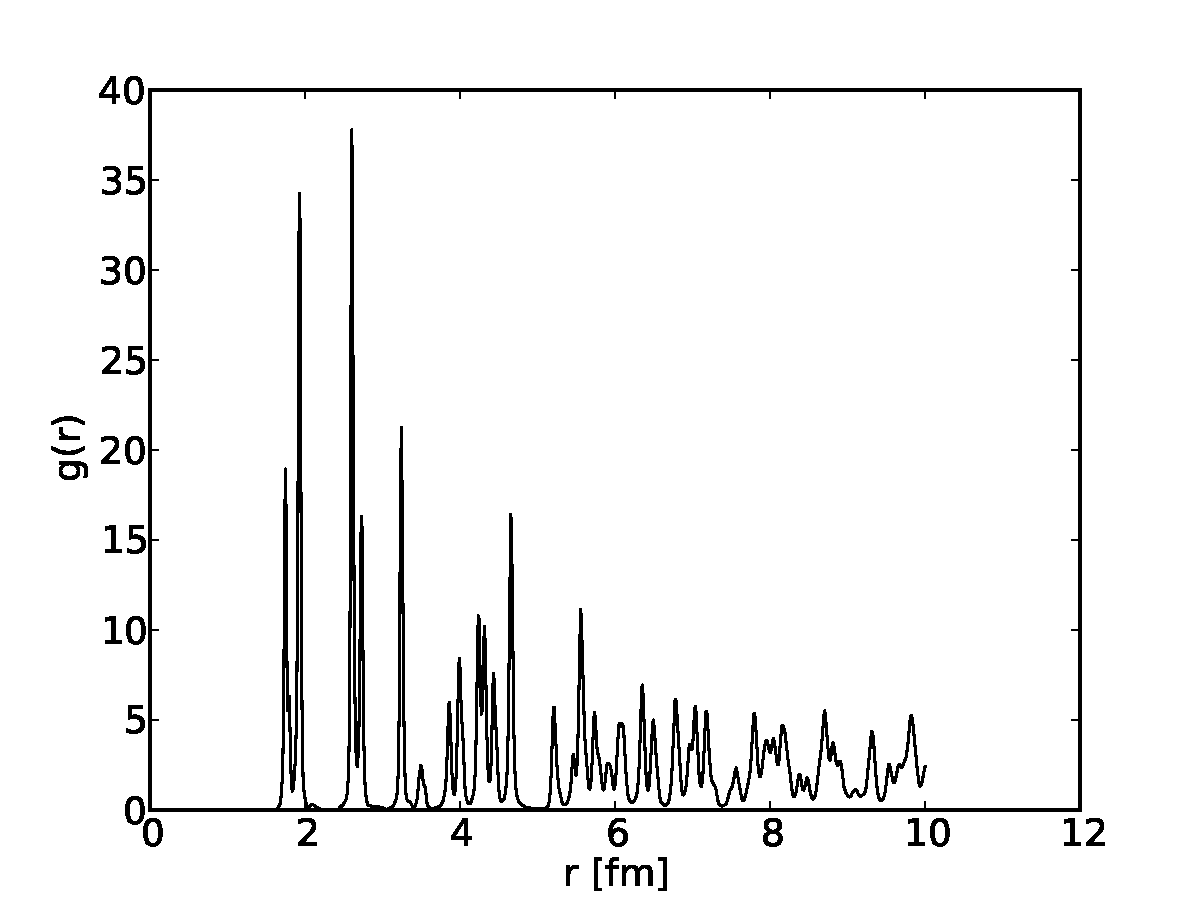
\includegraphics[width=\columnwidth]{coulomb/gofr-sing.pdf}
  \caption{Una lasagna}
\end{subfigure}
\caption{Ejemplos de la función distribución de pares para $\rho=0.05\,\text{fm}^{-3}$ y dos longitudes de apantallamiento:
  $\lambda=20\,\text{fm}$ y $\lambda=0\,\text{fm}$.
  Notar la diferencia en escalas en el eje $y$ para los dos gráficos.}
\label{fig:gofr}
\end{figure}

Como ejemplo, mostramos la función distribución de pares, $g(r)$, para $\rho=0.05\,\text{fm}^{-3}$ en la figura~\ref{fig:gofr}.
Aquí vemos que los primeros picos de la distribución se mantienen en las mismas distancias de $r=1.7\,\text{fm}, 1.9\,\text{fm}$ para ambas configuraciones.
Esto muestra que la estructura de rango corto está gobernada por el potencial nuclear incluso a $\lambda=20\,\text{fm}$, evidente simplemente al comparar los órdenes de magnitud de $V_{n-n}$ y $V_{\text{Coulomb}}$ para esos rangos.

Para la densidad $\rho=0.005\,\text{fm}^{-3}$, para longitudes de apantallamiento $\lambda<10\,\text{fm}$, hay un solo \emph{gnocchi}.
Sin embargo, cuando aumentamos de $\lambda=15\,\text{fm}$ a $\lambda=20\,\text{fm}$ para $\rho=0.005\,\text{fm}^{-3}$, aunque cualitativamente vemos el mismo comportamiento (ambos muestran \emph{gnocchi}), el tamaño promedio de los fragmentos es diferente para estos dos valores, de ahí la diferencia observada en las funcionales de Minkowski.
Para estudiar este resultado, graficamos el tamaño de los \emph{gnocchi} como función de $\lambda$ en la figura~\ref{fig:gnocchi_mass}.
Vemos que, cuando tenemos en cuenta la varianza en la distribución de masa, se mantiene estable para $\lambda\geq20\,\text{fm}$.
El error relativo promedio del gráfico es $e\approx8\%$.

\begin{figure}[h] %figure 3
\centering
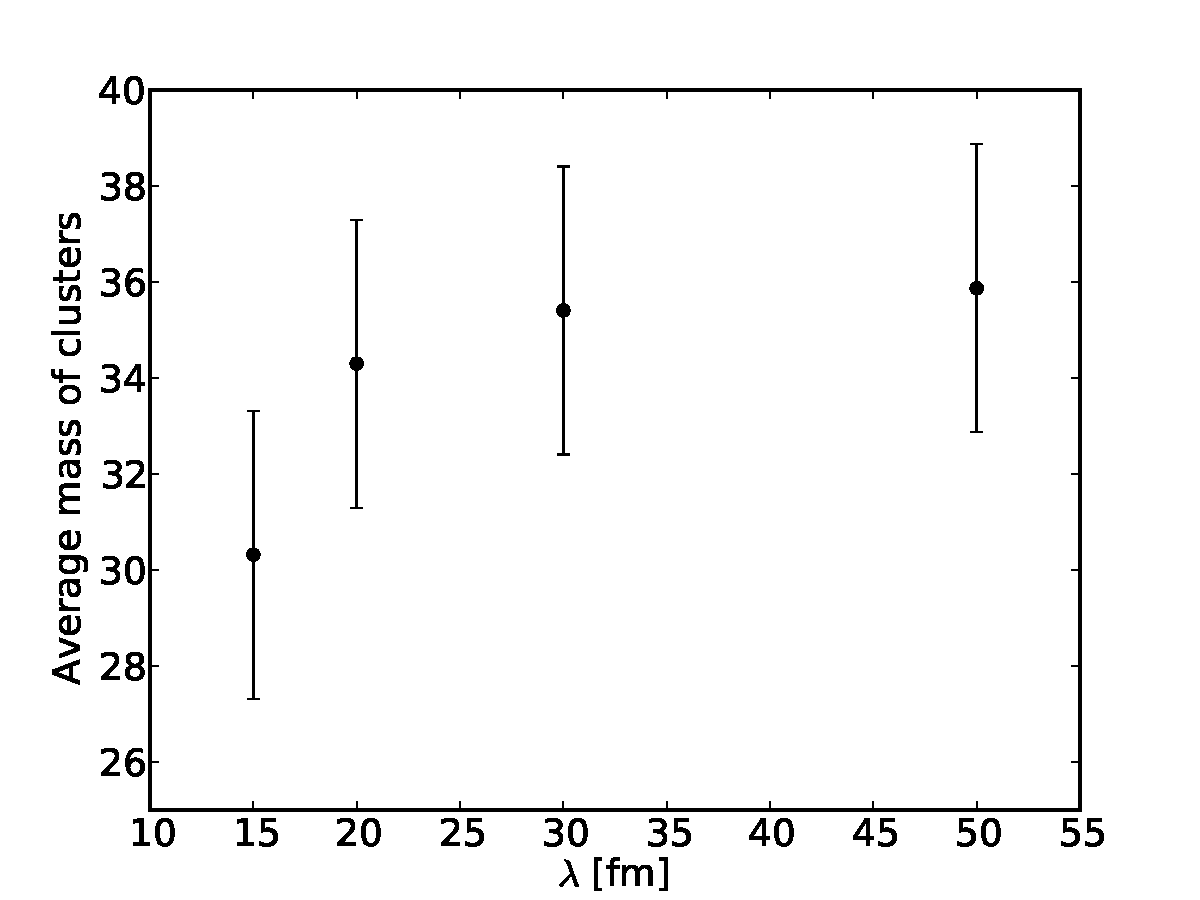
\includegraphics[width=0.7\columnwidth]{coulomb/gnocchi_mass}
\caption{Tamaño promedio de los \emph{gnocchi} dependiendo de la longitud de apantallamiento.}
\label{fig:gnocchi_mass}
\end{figure}

Podemos ver que aunque odas las estructuras sin Coulomb son alguna de las pastas conocidas, una vez que agregamos la interacción de Coulomb (haciendo $\lambda\neq0$), la \emph{pseudo-pasta} original de $\lambda=0$ se separa: de una estructura por celda a múltiples estructuras por celda.
Para valores intermedios a bajos de $\lambda < 20\,\text{fm}$, el efecto de las condiciones periódicas de contorno es todavía observable para algunas densidades y pueden aparece estructuras exóticas que no forman parte de las pastas usuales.

\section{El Régimen de Transición} \label{transition}

Vamos a estudiar ahora las estructuras halladas en el régimen de transición.

Tomemos, por ejemplo, la densidad más baja ($\rho=0.005\,\text{fm}^{-3}$).
Como podemos ver de la figura~\ref{fig:gnocchi}, para $\lambda=0$ sólo se forma una gota, como era de esperar.
Para $\lambda=10\,\text{fm}$ aparecen muchos \emph{gnocchi}, pero algunos de ellos se adhieren a sus vecinos, formando estructuras proladas de diferentes tamaños.
A pesar de que la interacción de Coulomb es ahora suficientemente grande como para partir la estructura monolítica hallada con $\lambda=0$ en varias, las gotas resultantes no son los usuales \emph{gnocchi} que se ordenan en una red regular, como sí lo son las halladas para $\lambda=20\,\text{fm}$.

\begin{figure}[h!]  \centering
  \begin{subfigure}[h!]{0.3\columnwidth}
    \centering
    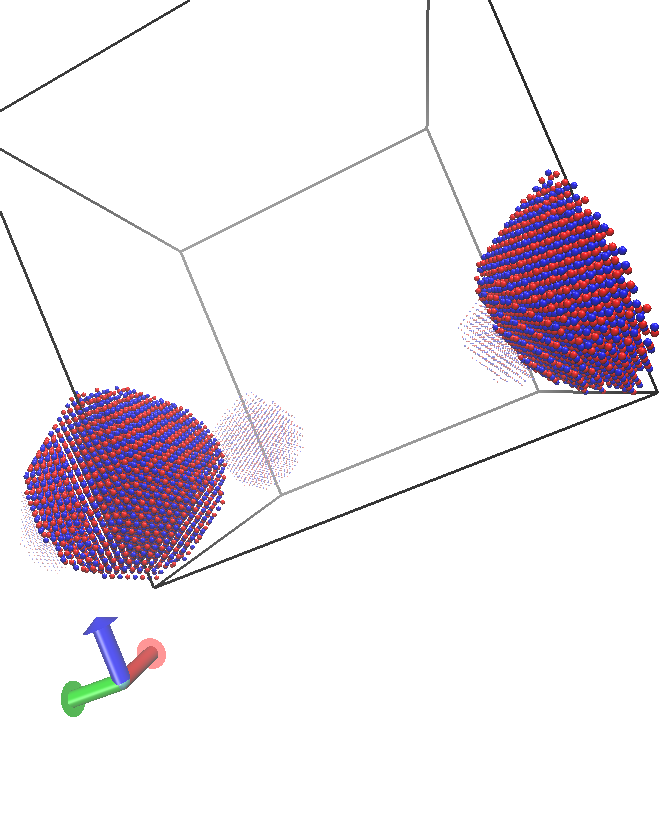
\includegraphics[width=\columnwidth]{coulomb/cou0-d0-005.png}
    \caption{$\lambda=0\,\text{fm}$}
  \end{subfigure}
  \begin{subfigure}[h!]{0.3\columnwidth}
    \centering
    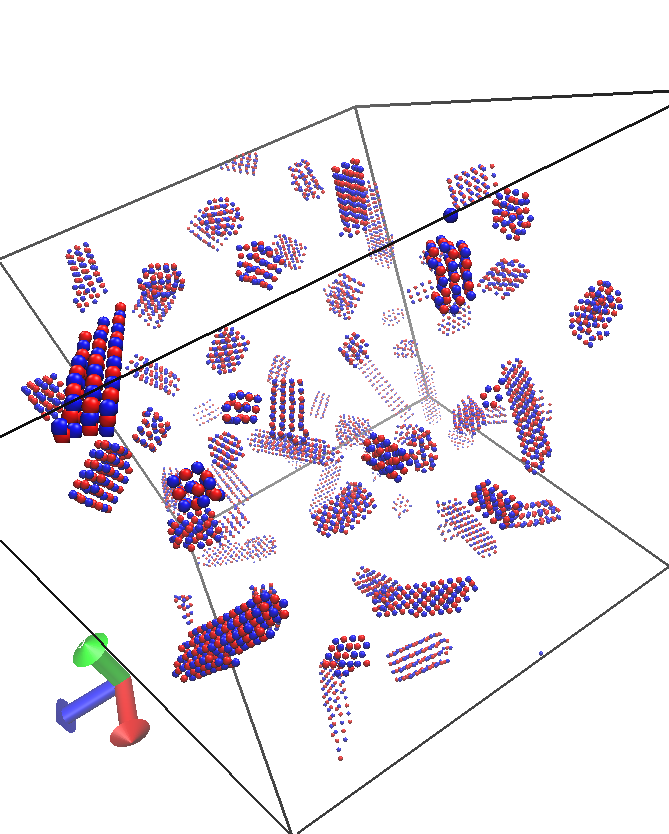
\includegraphics[width=\columnwidth]{coulomb/cou10-d0-005.png}
    \caption{$\lambda=10\,\text{fm}$}
  \end{subfigure}
  \begin{subfigure}[h!]{0.3\columnwidth}
    \centering
    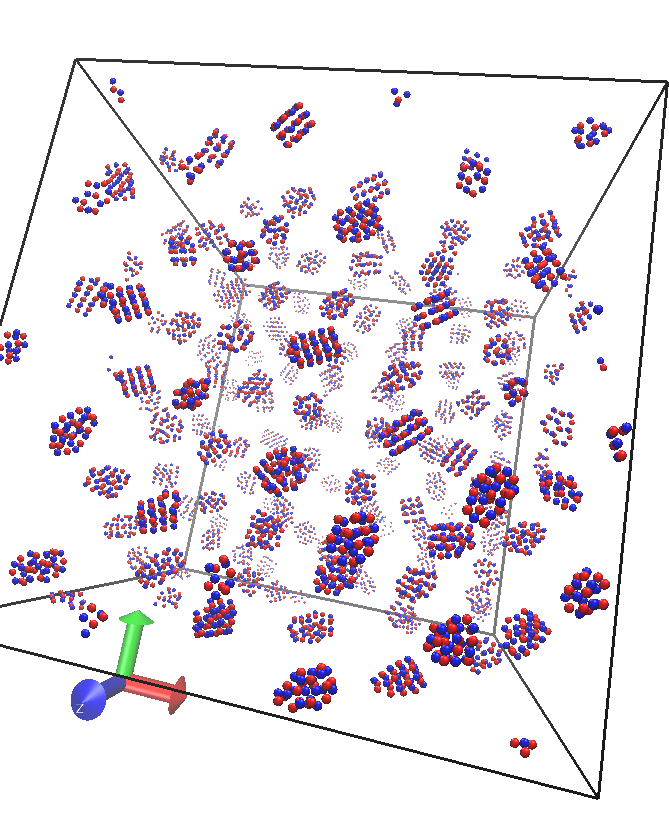
\includegraphics[width=\columnwidth]{coulomb/cou20-d0-005.png}
    \caption{$\lambda=20\,\text{fm}$}
  \end{subfigure}
  \caption{Diferentes estructuras halladas al variar la longitud de apantallamiento $\lambda$, para $\rho=0.005\text{fm}^{-3}$.
    En el régimen de transición hallamos, para $\lambda=10\,\text{fm}$, que la estructura se parte en varios fragmentos prolados, parecidos a \emph{spaghetti} cortados.}
  \label{fig:gnocchi}
\end{figure}


\section{Conclusiones}\label{concluding}

Estudiamos el efecto de la longitud de apantallamiento de la interacción de Coulomb en las simulaciones de materia de estrellas de neutrones a densidad comparables a las de la corteza de las estrellas de neutrones.
A lo largo de la literatura podemos encontrar que el valor de la longitud de apantallamiento en la aproximación de Thomas-Fermi es $\lambda\approx100\,\text{fm}$.
Para simulaciones basadas en partículas, debido a las limitaciones computacionales, este valor fue histórica y arbitrariamente reducido a $\lambda\approx10\,\text{fm}$, esperando mantener la fenomenología básica cuando se estudiaban sistemas pequeños.
Encontramos, sin embargo, que existe una longitud de apantallamiento crítica $\lambda_c$ a la cual la estructura del estado fundamental cambia drásticamente.
Para el potencial de Pandharipande en su parametrización Medium, yace entre $10\,\text{fm}$ y $15\,\text{fm}$ (dependiendo de la densidad).
Para $\lambda<\lambda_c$, la interacción de Coulomb apenas actúa y las estructuras no homogéneas que emergen de las simulaciones se deben a efectos de tamaño finito, como es evidente a partir de la presión negativa de estas estructuras y el hecho de que hay sólo una estructura por celda.
Para $\lambda>\lambda_c$ la presión se vuelve positiva y los sistemas presentan fluctuaciones de densidad a una escala menor que la de la celda, pero no con la forma de la pasta típica.
Este régimen de transición se caracteriza por grandes fluctuaciones en la superficie, ancho medio y característica de Euler $\chi$ de las estructuras.
Es recién para $\lambda=20\,\text{fm}$ que la morfología de las estructuras se estabiliza y deja de depender de $\lambda$.
Más aún, las estructuras en este régimen son las pastas usuales.

Debido a esto, creemos que se tiene que tomar extrema precaución cuando se elige un valor arbitrario de $\lambda$, ya que aunque algunos resultados a $\lambda=10\,\text{fm}$ pueden ser como la pasta esperada, los resultados obtenidos para esa elección particular de $\lambda$ pueden ser cualitativamente diferente de aquellos en la correcta aproximación de Thomas-Fermi.
En conclusión, encontramos que la elección de un buen valor para $\lambda$ que vuelve al sistema computable computacionalmente y puede adecuadamente recuperar la física de la aproximación de Thomas-Fermi no es una tarea trivial, y se necesita un estudio riguroso antes de escogerlo.
Un buen valor de $\lambda$ debe cumplir $\lambda>\lambda_c$, que depende del modelo utilizado para la interacción nuclear.


%  LocalWords:  Pandharipande Medium
